% !Mode:: "TeX:UTF-8"
% !TEX root = ..\thesis.tex
\chapter{计算实验及算法评估}
本章将对上一章的算法进行评估,通过设计相关计算实验,建立评价体系,具体评估各算法的效果及其适用规模。然后根据实验结果,为研究对象制定合适的调度方案。
\section{实验设计}
为了评估上一章所提出的算法的运行效果,以及给出所得调度方案,供决策者选择,所有的算法都用Python 语言编写,并在2.20GHz i3 CPU,5.84GB RAM,Windows 8 的个人计算机上运行。

实验设计分为两个主要部分,一个是装配生产信息的生成,包括订单数量、流水线数量、各订单切换准备时间、个订单进入系统时间及其所含作业的信息;另一个是相关参数的确定,包括迭代次数、禁忌列表长度的等。
\subsection{生产装配信息生成}
生产装配信息皆由随机数产生,主要包括订单及其作业的数量信息、时间信息及惩罚系数,需要给出适当的取值范围及分布。
\begin{asparaenum}
\item 数量信息
\suspend{asparaenum}

由\reft{tab:2jobshopinfo},设计实验中的流水线的数量$m$分别为$5,6,7$,订单品种数量的范围是$[29,777]$,据此可以设计合理的订单数量$n$分别为$20,30,50,70,100,150,200,300,500,750,1000$,再根据大批量的特点,可以设置订单中作业的批量范围为$(1000,2000)$。
\resume{asparaenum}
\item 时间信息
\suspend{asparaenum}

出于保护该公司的生产能力数据,实验中所采用的时间单位是经变换过的$tu$,由于每个订单的作业批量都比较大,所以订单中的作业处理时间单位为$1/500\ tu$。订单中的作业处理时间服从参数$\alpha = 5$的负指数分布,订单到达系统的时间间隔服从参数$\lambda = 3$的泊松分布
\resume{asparaenum}
\item 惩罚系数与优先系数
\end{asparaenum}

多品种多装配线轮番装配调度优化模型的目标函数\eqref{equ:objmain}中,延迟完成的订单有惩罚系数$wt$,订单的完成有优先系数$wc$,考虑插单的模型也有类似的这两类系数,皆由随机数产生。与模型中不同的是,由于订单中的批量增多,这些系数若满足求和为$1$的约束使得每个系数的值都很小,不利计算的准确性,而同时成倍扩大不影响调度的结果,所以这些系数不作求和为$1$的处理。

实验信息数据生成的代码见附录(experiment\_data.py),生成的数据在目录(.\textbackslash data\textbackslash)中,举例来说,$20$件订单的数据所含内容\footnote{本课题提出的两个模型使用相同的数据,考虑插单的模型将用到进入系统时间$r_j$}如\reft{tab:20itemsdata}所示。
\begin{table}[h]
  \centering
  \caption{$20$件订单的实验信息数据}
    \begin{tabular}{ccccccc}
     	&	&	&	&	&	&\multicolumn{1}{r}{单位:$tu$}\\
    \toprule
    订单序号 & 装配时间 & 进入系统时刻 & 切换准备时间& 约定工期 & 主要目标权重 & 次要目标权重 \\
    ($j$) & ($p_j$) & ($r_j$) &($s_j$) &($d_j$) &($w_{(t)}$) & ($w_c$) \\
    \midrule
    1     & 23    & 56    & 7     & 100   & 15    & 2 \\
    2     & 40    & 30    & 1     & 116   & 8     & 3 \\
    3     & 36    & 20    & 7     & 98    & 10    & 4 \\
    4     & 25    & 4     & 2     & 49    & 12    & 10 \\
    5     & 17    & 5     & 5     & 37    & 11    & 2 \\
    6     & 28    & 42    & 1     & 101   & 2     & 7 \\
    7     & 20    & 44    & 6     & 87    & 8     & 10 \\
    8     & 21    & 63    & 8     & 105   & 12    & 9 \\
    9     & 15    & 40    & 2     & 71    & 2     & 7 \\
    10    & 18    & 10    & 6     & 43    & 7     & 6 \\
    11    & 30    & 6     & 7     & 70    & 14    & 7 \\
    12    & 20    & 2     & 8     & 36    & 4     & 1 \\
    13    & 16    & 46    & 1     & 79    & 3     & 4 \\
    14    & 35    & 36    & 4     & 112   & 8     & 6 \\
    15    & 31    & 52    & 4     & 109   & 14    & 7 \\
    16    & 24    & 27    & 3     & 70    & 13    & 5 \\
    17    & 19    & 62    & 2     & 96    & 6     & 3 \\
    18    & 35    & 13    & 3     & 91    & 12    & 5 \\
    19    & 31    & 2     & 8     & 62    & 4     & 10 \\
    20    & 24    & 60    & 6     & 101   & 3     & 8 \\
    \bottomrule
    \end{tabular}
  \label{tab:20itemsdata}
\end{table}

\subsection{相关参数确定}
使用调度规则(ATC/ATCS)的交替算法所含的相关参数为交替次数$NR$,由于该算法收敛速度很快,该参数无需特别设定,一般取$NR = 30$就基本稳定在最佳的两个结果之间交替。

实验中涉及到禁忌搜索的部分,其相关参数包括迭代次数、禁忌列表长度等,迭代次数增多会增大改进解的机率,但是会使得运算时间变长,禁忌列表过长会浪费迭代次数,过短则可能跳不出局部最优。所以需要在实验前需要设定恰当的参数,以订单数量$n = 100$为例,运用虚拟序列禁忌搜索算法\refa{alg:basicvirtual},决策权重$\lambda_t =0.6, \lambda_c = 0.4$,流水线数量$m = 5$时,在初始解生成迭代次数$N_{init} = 20$的情况下,禁忌列表长度与初始解的函数值关系如\reff{fig:100NLwithGoal}所示。
\begin{figure}[h]
\centering
\subfloat[禁忌列表长度]{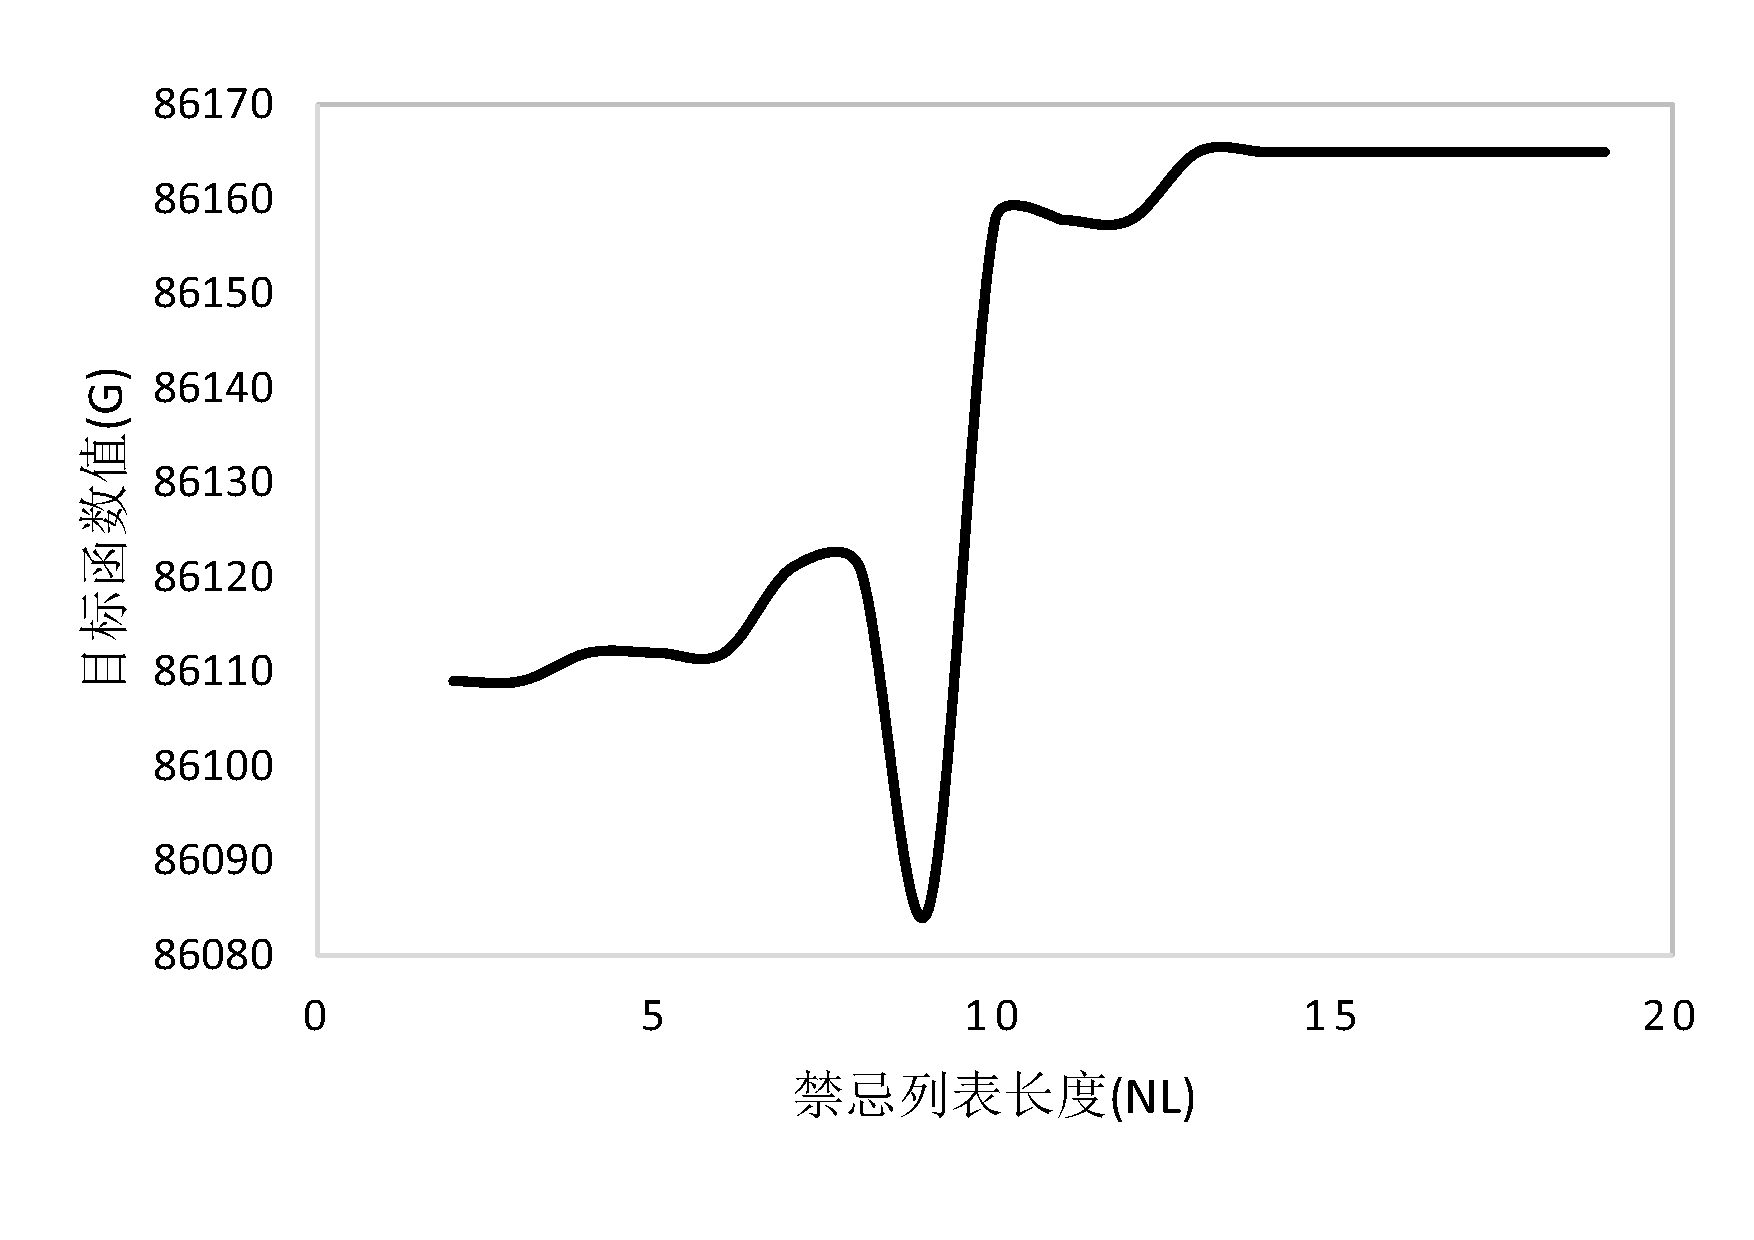
\includegraphics[height= 8.2cm,angle = -90]{NL_100}\label{fig:100NLwithGoal}}
\subfloat[迭代次数]{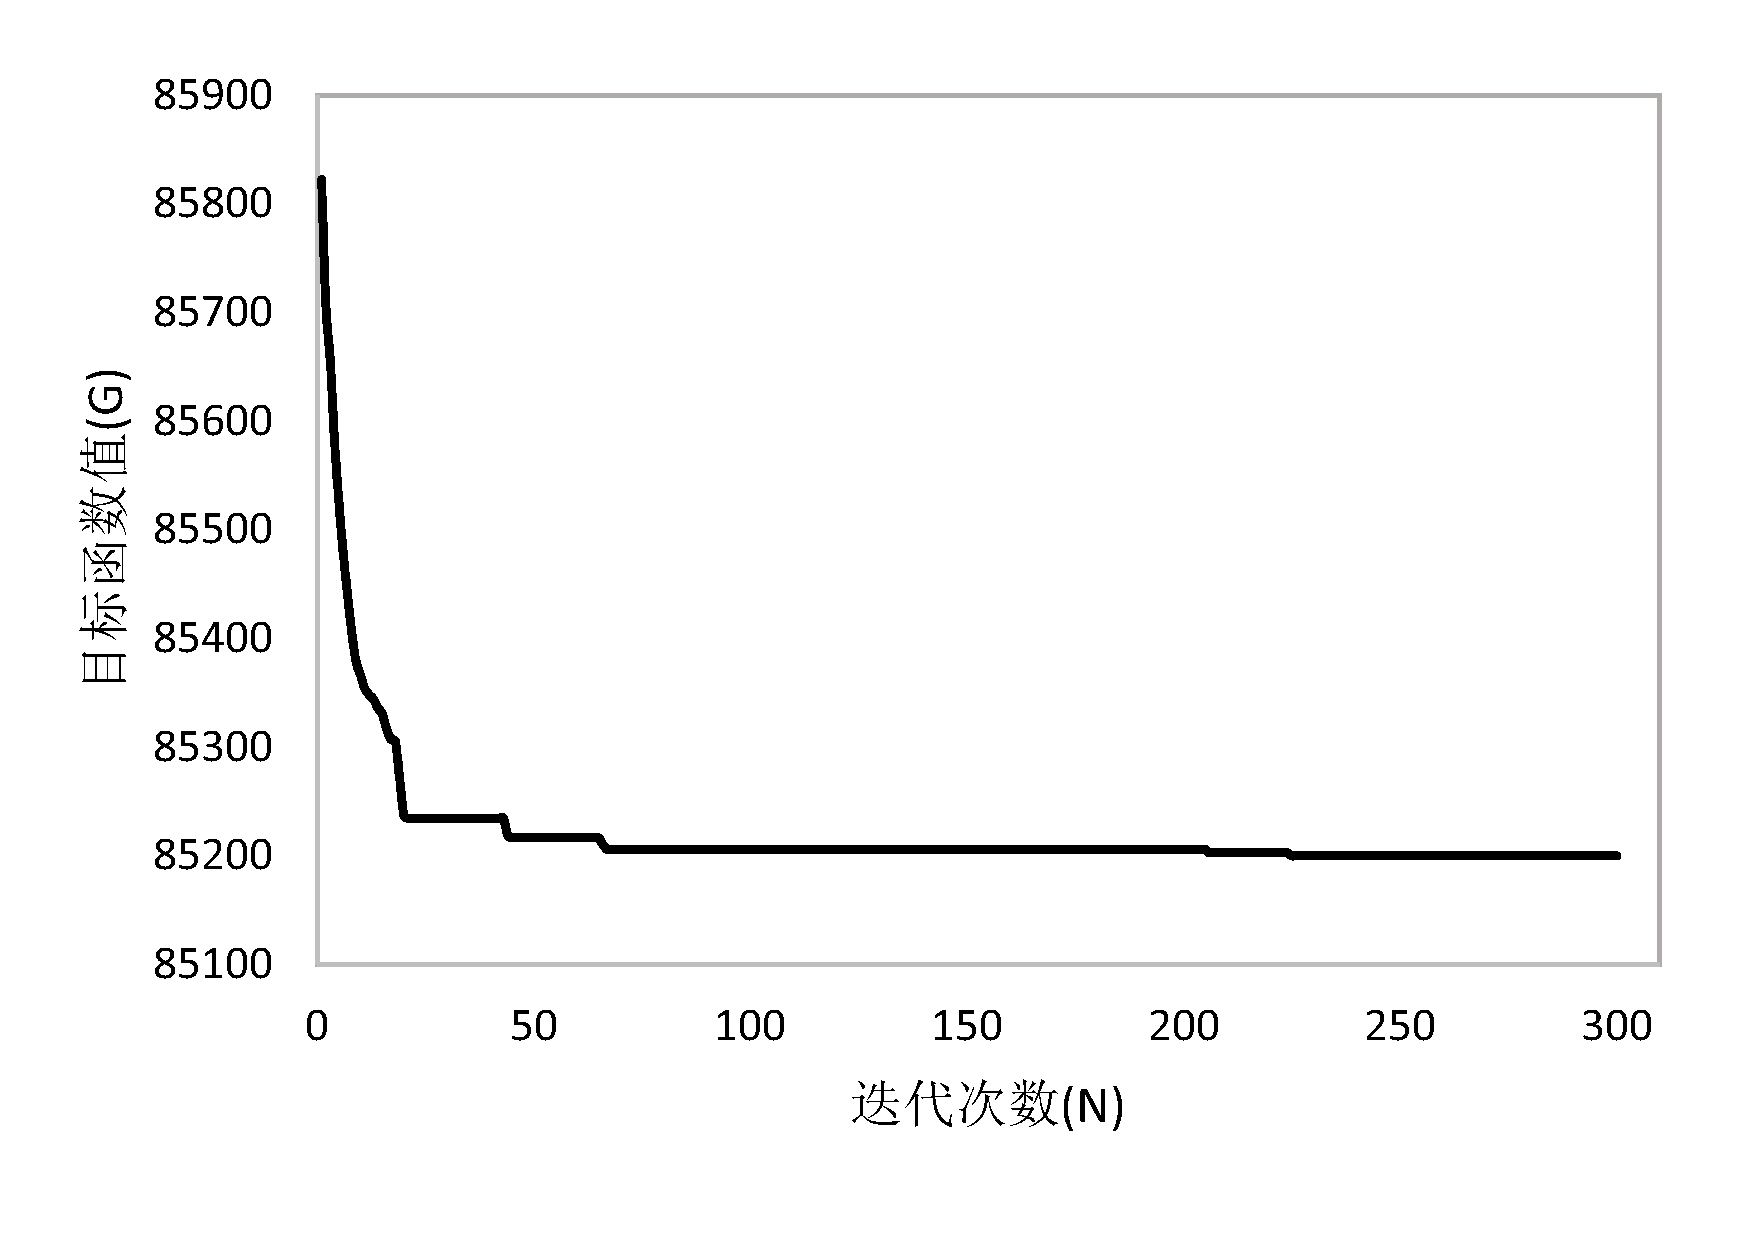
\includegraphics[height= 8.2cm,angle = -90]{N_100}\label{fig:100NwithGoal}}
\caption{$100$件订单的目标函数值和相关参数的关系}
\end{figure}

可以看出$NL = 9$是最佳列表长度,确定该值后,生成目标函数值与迭代次数的关系,如\reff{fig:100NwithGoal}所示。
虽然随着迭代次数的增加,目标函数值仍然会减少,其减少幅度不大,并且运算时间增加很多,所以取迭代次数$N = 70$是较为适宜的\footnote{实际上$\left. G\right|_{N=70} = 85206, \left. G\right|_{N=300} = 85200.2$,两者相差仅$0.0068\%$}。

以此类推,可以确定不同问题规模下的这两个参数的值\footnote{经测试,不用决策环境$(\lambda_1, \lambda_2, \sigma)$下,禁忌列表长度$NL$和迭代次数$N$基本不变,所以这两个参数适用于不同的决策环境下},多品种多装配线轮番装配调度优化模型和考虑插单的多品种多装配线轮番装配调度优化模型相关参数设定结果分别如和所示。
\begin{table}[htbp]
  \centering
  \caption{Add caption}
    \begin{tabular}{ccccccccccccc}
    \toprule
    \multicolumn{2}{c}{\multirow{2}[0]{*}{参数}} & \multicolumn{11}{c}{订单数量} \\
        \multicolumn{2}{c}{} & $20 $   & $30$    & $50$    & $70$    & $100$   & $150 $  & $200$   & $300$   & $500$   & $750$   & $1000$ \\
      \midrule
    \multirow{2}[0]{*}{$m=5$} & $N$     & $3$     & $16$    & $65$    & $30$    & $70$    & $100$   & $1850$  & $1700$  & $1000$  & $150$   & $500$ \\
          & $NL$    & $2$     & $2$     & $8$     & $6$     & $9$     & $29$    & $61$    & $138$   & $164$   & $152$   & $90$ \\
    \multirow{2}[0]{*}{$m=6$} & $N$     & $14$    & $10$    & $25$    & $60$    & $130$   & $200$   & $850$   & $420$   &  $350 $     &  $650 $     &$440$  \\
          & $NL$    & $2$     & $2$     & $2$     & $6$     & $20$    & $31$    & $52$    & $105$   & $190$   & $220$   & $312$ \\
    \multirow{2}[0]{*}{$m=7$} & $N$     & $8$     & $13$    &$ 60    $&$ 55    $&$ 19    $&$ 200   $&$ 320   $&$ 275   $&$80       $&$      700 $&$80  $\\
          &$ NL    $&$ 2     $&$ 2     $&$ 4     $&$ 14    $&$ 6     $&$ 21    $&$ 26    $&$ 48    $&$ 160   $&$ 227   $&$ 174 $\\
    \bottomrule
    \end{tabular}%
  \label{tab:addlabel}%
\end{table}%

\begin{table}[htbp]
  \centering
  \caption{Add caption}
    \begin{tabular}{cccccccccccccc}
    \toprule
    $m $    & \multicolumn{2}{c}{参数} & 20    & 30    & 50    & 70    & 100   & 150   & 200   & 300   & 500   & 750   & 1000 \\
    \midrule
    \multirow{4}[0]{*}{5} & \multirow{2}[0]{*}{基本模型} & $N$    & 2     & 2     & 8     & 6     & 9     & 13    & 27    & 18    &       &       &  \\
          &       & $NL$    &       &       &       &       &       &       &       &       &       &       &  \\
          & \multirow{2}[0]{*}{插单模型} & $N$    & 2     &       &       &       &       &       &       &       &       &       &  \\
          &       & $NL$    &       &       &       &       &       &       &       &       &       &       &  \\
    \multirow{4}[0]{*}{6} & \multirow{2}[0]{*}{基本模型} & $N$    & 2     &       &       &       &       &       &       &       &       &       &  \\
          &       & $NL$    &       &       &       &       &       &       &       &       &       &       &  \\
          & \multirow{2}[0]{*}{插单模型} & $N$    & 2     &       &       &       &       &       &       &       &       &       &  \\
          &       & $NL$    &       &       &       &       &       &       &       &       &       &       &  \\
    \multirow{4}[0]{*}{7} & \multirow{2}[0]{*}{基本模型} & $N$    & 2     &       &       &       &       &       &       &       &       &       &  \\
          &       & $NL$    &       &       &       &       &       &       &       &       &       &       &  \\
          & \multirow{2}[0]{*}{插单模型} & $N$    & 2     &       &       &       &       &       &       &       &       &       &  \\
          &       & $NL$    &       &       &       &       &       &       &       &       &       &       &  \\
    \bottomrule
    \end{tabular}%
  \label{tab:addlabel}%
\end{table}%
可以看出,迭代次数和禁忌列表长度和问题的规模有一定的正相关关系,问题规模越大,这两者的值也越大,但这两个参数主也和订单的实验信息数据特点有关。
 
\section{结果及评估}
\subsection{实验结果示例及说明}
确定实验所需订单信息数据以及算法相关的参数,运行编写的算法程序,可以得到实验结果。实验结果由目标函数值$G$和所得调度序列$S$组成,以模型$1$ 为例,示例订单量$n = 20$,其实验信息数据如\ref{tab:20itemsdata}所示,在决策参数$\lambda_1 = 0.6, \lambda_2 = 0.4$的环境下,分别采用Cyc -- ATC 算法、Cyc -- Tabu 算法和Vtr -- Tabu 算法,根据 选择相关参数,所得结果列入中。
\begin{table}[htbp]
  \centering
  \caption{Add caption}
    \begin{tabular}{cccl}
    \toprule
    算法    & 目标函数值($G$) & \multicolumn{2}{c}{流水线调度安排} \\
    \midrule
    \multirow{5}[2]{*}{Cyc -- ATC} & \multirow{5}[2]{*}{$3978.8$} & $1$     &$\xymatrix{10 \ar[r] & 18 \ar[r] & 14 \ar[r] & 6}$\\
          &       & $2$     &  $\xymatrix{11 \ar[r] & 7 \ar[r] & 2}$\\
          &       & $3$     &  $\xymatrix{16 \ar[r] & 15 \ar[r] & 13 \ar[r] & 9}$\\
          &       & $4$     &  $\xymatrix{4 \ar[r] & 8 \ar[r] & 17 \ar[r] & 12 \ar[r]&20}$\\
          &       & $5$     &  $\xymatrix{5 \ar[r] & 1 \ar[r] & 3 \ar[r] & 19}$\\
     \hline
    \multirow{5}[2]{*}{Cyc -- Tabu} & \multirow{5}[2]{*}{$3478.8$} & $1$     &  $\xymatrix{10 \ar[r] & 6 \ar[r] & 18 \ar[r] & 14}$\\
          &       & $2$     & $\xymatrix{7 \ar[r] & 11 \ar[r] & 20 \ar[r] & 2}$ \\
          &       & $3$     &  $\xymatrix{9 \ar[r] & 13 \ar[r] & 16 \ar[r] & 15}$\\
          &       & $4$     &  $\xymatrix{4 \ar[r] & 8 \ar[r] & 17 \ar[r] & 12}$\\
          &       & $5$     &  $\xymatrix{5 \ar[r] & 19 \ar[r] & 1 \ar[r] & 3}$\\
       \hline
    \multirow{5}[2]{*}{Vtr -- Tabu} & \multirow{5}[2]{*}{$3329.2$} & $1$     &  $\xymatrix{10 \ar[r] & 20 \ar[r] & 18 \ar[r] & 2}$\\
          &       & $2$     & $\xymatrix{7 \ar[r] & 11 \ar[r] & 14 }$ \\
          &       & $3$     &  $\xymatrix{9 \ar[r] & 13 \ar[r] & 16 \ar[r] & 15\ar[r]&6}$\\
          &       & $4$     &  $\xymatrix{4\ar[r] & 8 \ar[r] & 3 \ar[r] & 12}$\\
          &       & $5$     &  $\xymatrix{5 \ar[r] & 19 \ar[r] & 1 \ar[r] & 17}$\\
    \bottomrule
    \end{tabular}%
  \label{tab:addlabel}%
\end{table}%
其调度安排如\reff{fig:20items3algorithms}所示。
%% !Mode:: "TeX:UTF-8"
% !TEX root = ..\thesis.tex
\begin{figure}
\centering
\subfloat[原始调度结果\label{fig:orginschedule}]{\resizebox{12.7cm}{!}{\begin{tikzpicture}
\fill[blue!20!] (116mm,2.5mm) rectangle (141mm,7.5mm)
			 (105mm,12.5mm) rectangle (106mm,17.5mm)
			  (43mm,22.5mm) rectangle (52mm,27.5mm) 
			  (70mm,22.5mm) rectangle (106mm,27.5mm)
			  (112mm,32.5mm) rectangle (118mm,37.5mm)
			   (96mm,42.5mm) rectangle (98mm,47.5mm)
			    (101mm,42.5mm) rectangle (128mm,47.5mm);
\draw (70mm,-7mm) node{$G = 6227.2$};
\draw [->,very thick] (0,0) -- (140mm,0);
\draw (25mm,0) -- (25mm,1mm) (25mm,-3mm) node{$25$} (50mm,0) -- (50mm,1mm) (50mm,-3mm) node{$50$} (75mm,0) -- (75mm,1mm) (75mm,-3mm) node{$70$}  (100mm,0) -- (100mm,1mm) (100mm,-3mm) node{$100$} (125mm,0) -- (125mm,1mm) (125mm,-3mm) node{$125$} (143mm,0) node{$tu$};
\draw [very thick] (0,0) -- (0,50mm) (0.4,53mm) node{流水线};
\draw [thick] (-2mm,5mm) node{$1$} (0,2.5mm) rectangle (27mm,7.5mm) rectangle (70mm,2.5mm) rectangle (100mm,7.5mm) rectangle (141mm,2.5mm);
\draw [thick] (-2mm,15mm) node{$2$} (0,12.5mm) rectangle (22mm,17.5mm) rectangle (48mm,12.5mm) rectangle (77mm,17.5mm) rectangle (106mm,12.5mm);
\draw [thick] (-2mm,25mm) node{$3$} (0,22.5mm) rectangle (28mm,27.5mm) rectangle (52mm,22.5mm) rectangle (89mm,27.5mm) rectangle (106mm,22.5mm) ;
\draw [thick] (-2mm,35mm) node{$4$} (0,32.5mm) rectangle (27mm,37.5mm) rectangle (44mm,32.5mm) rectangle (79mm,37.5mm) rectangle (118mm,32.5mm); 
\draw [thick] (-2mm,45mm) node{$5$} (0,42.5mm) rectangle (39mm,47.5mm) rectangle (77mm,42.5mm) rectangle (98mm,47.5mm) rectangle (128mm, 42.5mm);
\draw (19.5mm,45mm) node{$19$} (58mm,45mm) node{$18$} (87.5mm,45mm) node{$17$} (113mm,45mm) node{$20$} ;
\draw (13.5mm,35mm) node{$16$} (35.5mm,35mm) node{$13$} (61.5mm,35mm) node{$15$} (98.5mm,35mm) node{$14$} ;
\draw (14mm,25mm) node{$12$} (40mm,25mm) node{$10$} (70.5mm,25mm) node{$11$} (97.5mm,25mm) node{$9$};
\draw (11mm,15mm) node{$5$} (35mm,15mm) node{$7$} (62.5mm,15mm) node{$6$} (91.5mm,15mm) node{$8$};
\draw (13.5mm,5mm) node{$4$} (48.5mm,5mm) node{$3$} (85mm,5mm) node{$1$} (120.5mm,5mm) node{$2$};
\end{tikzpicture}}}\\[-3pt]
\subfloat[Cyc -- ATC 算法调度结果]{\resizebox{12.7cm}{!}{\begin{tikzpicture}
\fill[blue!20!] (101mm,2.5mm) rectangle (130mm,7.5mm) (79mm,22.5mm) rectangle (96mm,27.5mm) (77mm,32.5mm) rectangle (105mm,37.5mm) (110mm,32.5mm)rectangle(135mm,37.5mm) (95mm,42.5mm) rectangle (134mm,47.5mm) ;
\draw (70mm,-7mm) node{$G = 6136$};
\draw [->,very thick] (0,0) -- (140mm,0);
\draw (25mm,0) -- (25mm,1mm) (25mm,-3mm) node{$25$} (50mm,0) -- (50mm,1mm) (50mm,-3mm) node{$50$} (75mm,0) -- (75mm,1mm) (75mm,-3mm) node{$70$}  (100mm,0) -- (100mm,1mm) (100mm,-3mm) node{$100$} (125mm,0) -- (125mm,1mm) (125mm,-3mm) node{$125$} (143mm,0) node{$tu$};
\draw [very thick] (0,0) -- (0,50mm) (0.4,53mm) node{流水线};
\draw [thick] (-2mm,5mm) node{$1$} (0,2.5mm) rectangle (24mm,7.5mm) rectangle (62mm,2.5mm) rectangle (101mm,7.5mm) rectangle (130mm,2.5mm);
\draw [thick] (-2mm,15mm) node{$2$} (0,12.5mm) rectangle (37mm,17.5mm) rectangle (63mm,12.5mm) rectangle (104mm,17.5mm);
\draw [thick] (-2mm,25mm) node{$3$} (0,22.5mm) rectangle (27mm,27.5mm) rectangle (62mm,22.5mm) rectangle (79mm,27.5mm) rectangle (96mm,22.5mm) ;
\draw [thick] (-2mm,35mm) node{$4$} (0,32.5mm) rectangle (27mm,37.5mm) rectangle (56mm,32.5mm) rectangle (77mm,37.5mm) rectangle (105mm,32.5mm) rectangle(135mm,37.5mm);
\draw [thick] (-2mm,45mm) node{$5$} (0,42.5mm) rectangle (22mm,47.5mm) rectangle (52mm,42.5mm) rectangle (95mm,47.5mm) rectangle (134mm, 42.5mm);
\draw (11mm,45mm) node{$5$} (37mm,45mm) node{$1$} (73.5mm,45mm) node{$3$} (114.5mm,45mm) node{$19$} ;
\draw (13.5mm,35mm) node{$4$} (41.5mm,35mm) node{$8$} (66.5mm,35mm) node{$17$} (91mm,35mm) node{$12$} (120mm,35mm) node{$20$};
\draw (13.5mm,25mm) node{$16$} (44.5mm,25mm) node{$15$} (70.5mm,25mm) node{$13$} (87.5mm,25mm) node{$9$};
\draw (18.5mm,15mm) node{$11$} (50mm,15mm) node{$7$} (83.5mm,15mm) node{$2$} ;
\draw (12mm,5mm) node{$10$} (43mm,5mm) node{$18$} (79.5mm,5mm) node{$14$} (115.5mm,5mm) node{$6$};
\end{tikzpicture}}}\\[-3pt]
\subfloat[Cyc -- Tabu 算法调度结果]{\resizebox{12.7cm}{!}{\begin{tikzpicture}
\fill[blue!20!] (101mm,2.5mm) rectangle (130mm,7.5mm) (101mm,22.5mm)rectangle(126mm,27.5mm) (77mm,32.5mm) rectangle (105mm,37.5mm) (95mm,42.5mm) rectangle (134mm,47.5mm) ;
\draw [->,very thick] (0,0) -- (140mm,0);
\draw (25mm,0) -- (25mm,1mm) (25mm,-3mm) node{$25$} (50mm,0) -- (50mm,1mm) (50mm,-3mm) node{$50$} (75mm,0) -- (75mm,1mm) (75mm,-3mm) node{$70$}  (100mm,0) -- (100mm,1mm) (100mm,-3mm) node{$100$} (125mm,0) -- (125mm,1mm) (125mm,-3mm) node{$125$} (143mm,0) node{$tu$};
\draw (70mm,-7mm) node{$G = 5638.4$};
\draw [very thick] (0,0) -- (0,50mm) (0.4,53mm) node{流水线};
\draw [thick] (-2mm,5mm) node{$1$} (0,2.5mm) rectangle (24mm,7.5mm) rectangle (62mm,2.5mm) rectangle (101mm,7.5mm) rectangle (130mm,2.5mm);
\draw [thick] (-2mm,15mm) node{$2$} (0,12.5mm) rectangle (26mm,17.5mm) rectangle (63mm,12.5mm) rectangle (104mm,17.5mm) ;
\draw [thick] (-2mm,25mm) node{$3$} (0,22.5mm) rectangle (17mm,27.5mm) rectangle (34mm,22.5mm) rectangle (61mm,27.5mm) rectangle (96mm,22.5mm) rectangle (126mm,27.5mm);
\draw [thick] (-2mm,35mm) node{$4$} (0,32.5mm) rectangle (27mm,37.5mm) rectangle (56mm,32.5mm) rectangle (77mm,37.5mm) rectangle (105mm,32.5mm);
\draw [thick] (-2mm,45mm) node{$5$} (0,42.5mm) rectangle (22mm,47.5mm) rectangle (52mm,42.5mm) rectangle (95mm,47.5mm) rectangle (134mm, 42.5mm);
\draw (11mm,45mm) node{$5$} (37mm,45mm) node{$1$} (73.5mm,45mm) node{$3$} (114.5mm,45mm) node{$19$} ;
\draw (13.5mm,35mm) node{$4$} (41.5mm,35mm) node{$8$} (66.5mm,35mm) node{$17$} (91mm,35mm) node{$12$} ;
\draw (8.5mm,25mm) node{$9$} (25.5mm,25mm) node{$13$} (47.5mm,25mm) node{$16$} (78.5mm,25mm) node{$15$} (111mm,25mm) node{$20$};
\draw (13mm,15mm) node{$7$} (44.5mm,15mm) node{$11$}  (83.5mm,15mm) node{$2$};
\draw (12mm,5mm) node{$10$} (43mm,5mm) node{$18$} (81.5mm,5mm) node{$14$} (115.5mm,5mm) node{$6$} ;
\end{tikzpicture}}}\\[-3pt]
\subfloat[Vtr -- Tabu 算法调度结果]{\resizebox{12.7cm}{!}{\begin{tikzpicture}
\fill[blue!20!] (101mm,2.5mm) rectangle (113mm,7.5mm) (116mm,2.5mm)  (79mm,22.5mm) rectangle (118mm,27.5mm) (109mm,32.5mm) rectangle (137mm,37.5mm) (101mm,42.5mm) rectangle (129mm,47.5mm) ;
\draw [->,very thick] (0,0) -- (140mm,0);
\draw (25mm,0) -- (25mm,1mm) (25mm,-3mm) node{$25$} (50mm,0) -- (50mm,1mm) (50mm,-3mm) node{$50$} (75mm,0) -- (75mm,1mm) (75mm,-3mm) node{$70$}  (100mm,0) -- (100mm,1mm) (100mm,-3mm) node{$100$} (125mm,0) -- (125mm,1mm) (125mm,-3mm) node{$125$} (143mm,0) node{$tu$};
\draw (70mm,-7mm) node{$G = 5482.4$};
\draw [very thick] (0,0) -- (0,50mm) (0.4,53mm) node{流水线};
\draw [thick] (-2mm,5mm) node{$1$} (0,2.5mm) rectangle (24mm,7.5mm) rectangle (62mm,2.5mm) rectangle (83mm,7.5mm) rectangle (113mm,2.5mm);
\draw [thick] (-2mm,15mm) node{$2$} (0,12.5mm) rectangle (26mm,17.5mm) rectangle (63mm,12.5mm) rectangle (102mm,17.5mm);
\draw [thick] (-2mm,25mm) node{$3$} (0,22.5mm) rectangle (17mm,27.5mm) rectangle (44mm,22.5mm) rectangle (79mm,27.5mm) rectangle (118mm,22.5mm);
\draw [thick] (-2mm,35mm) node{$4$} (0,32.5mm) rectangle (27mm,37.5mm) rectangle (51mm,32.5mm) rectangle (68mm,37.5mm) rectangle (109mm,32.5mm) rectangle (137mm, 37.5mm);
\draw [thick] (-2mm,45mm) node{$5$} (0,42.5mm) rectangle (27mm,47.5mm) rectangle (70mm,42.5mm) rectangle (100mm,47.5mm) rectangle (129mm, 42.5mm);
\draw (13.5mm,45mm) node{$4$} (48.5mm,45mm) node{$3$} (85mm,45mm) node{$1$} (114.5mm,45mm) node{$6$} ;
\draw (11mm,35mm) node{$5$} (36.5mm,35mm) node{$8$} (59.5mm,35mm) node{$13$} (88.5mm,35mm) node{$2$} (123mm,35mm) node{$12$} ;
\draw (8.5mm,25mm) node{$9$} (30.5mm,25mm) node{$16$} (61.5mm,25mm) node{$15$} (98.5mm,25mm) node{$19$} ;
\draw (13mm,15mm) node{$7$} (44.5mm,15mm) node{$11$} (82.5mm,15mm) node{$14$} ;
\draw (12mm,5mm) node{$10$} (43mm,5mm) node{$18$} (72.5mm,5mm) node{$17$} (98mm,5mm) node{$20$};
\end{tikzpicture}}}
\caption{模型$1$下 $20$件订单原始调度结果和三种算法求解所得结果\label{fig:20items3algorithms}}
\end{figure}
从结果上来看,就该决策环境下,模型1 使用Vtr -- Tabu 算法可以得到较好调度结果。
\subsection{模型1}

\subsubsection{算法比较}
\subsubsection{权衡决策参数}
\begin{figure}[h]
\centering
\subfloat[$n = 1000$]{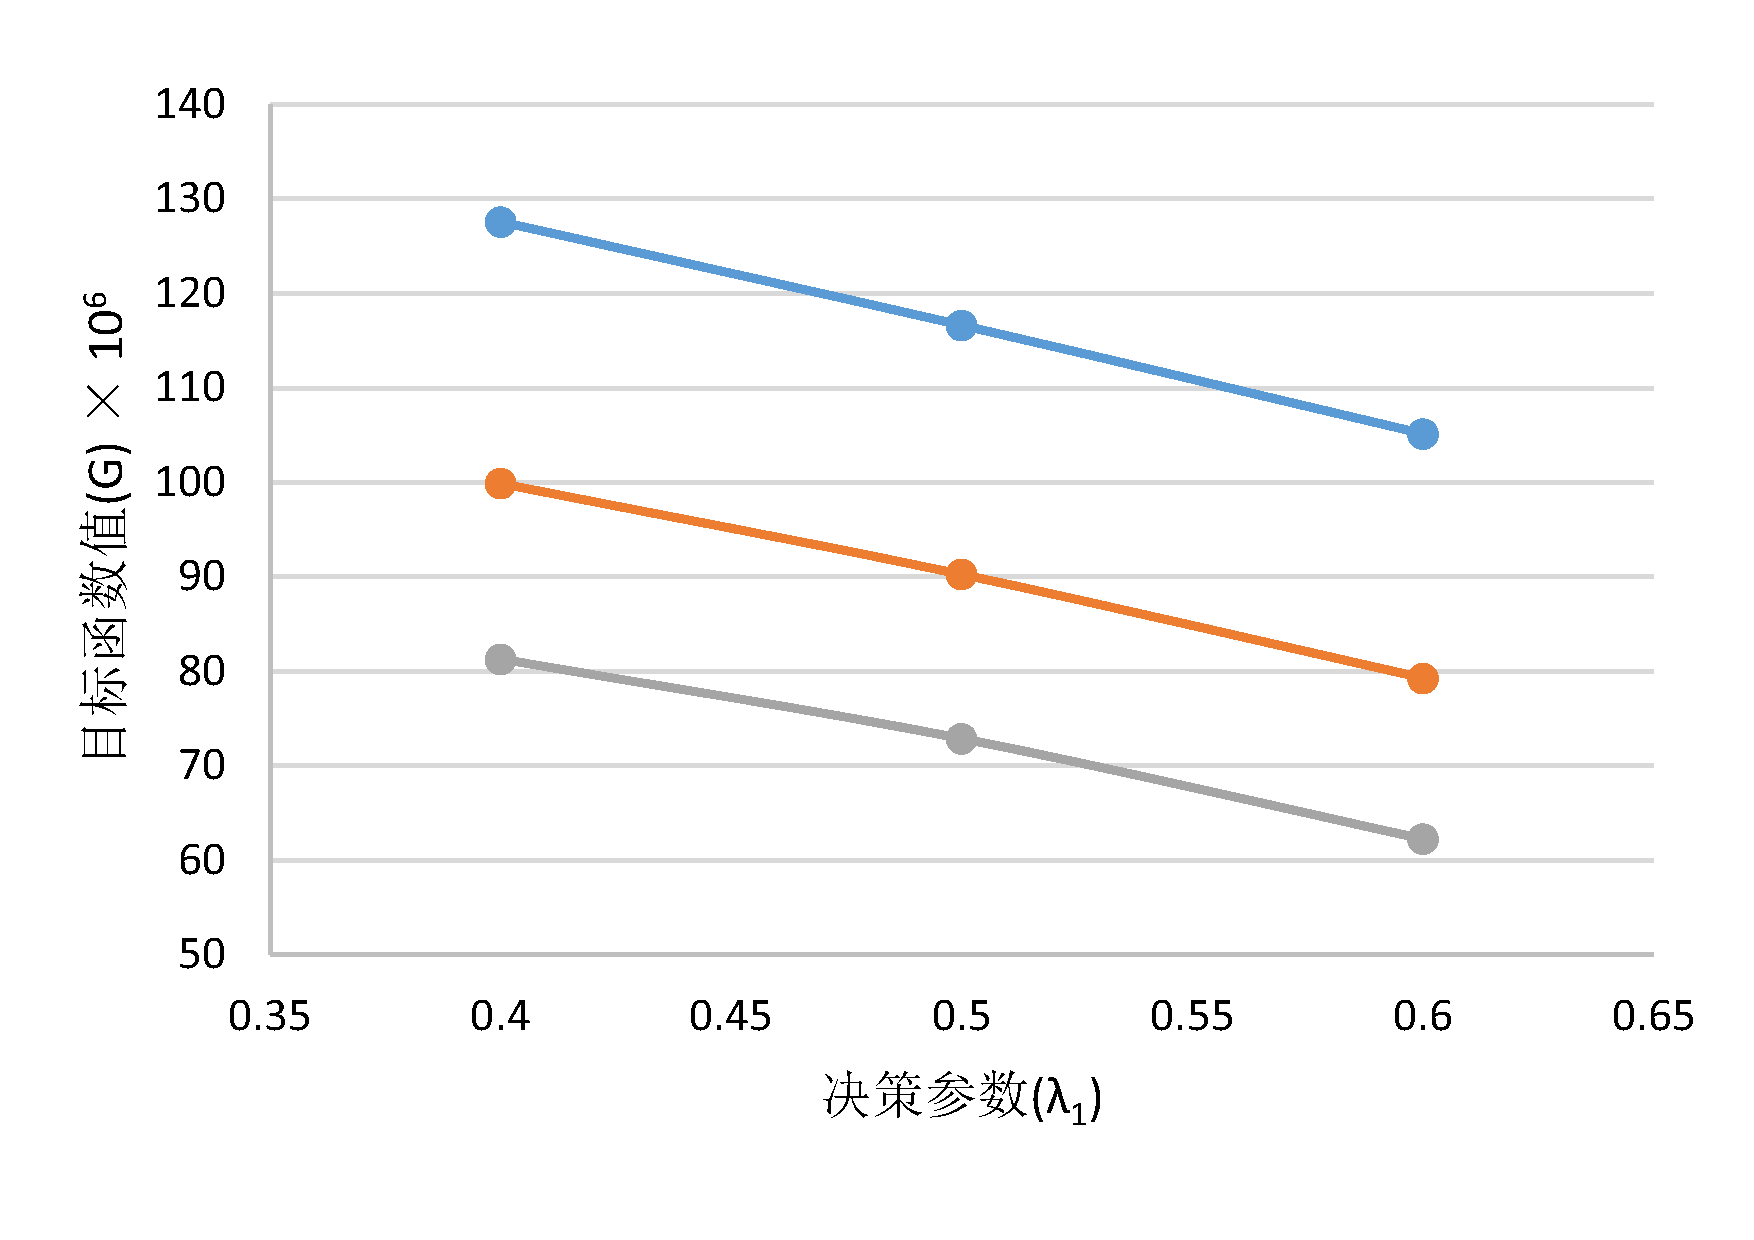
\includegraphics[height = 5.8cm, angle = -90,trim = 50 20 50 10]{alg_1_1000}}
\subfloat[$n = 750$]{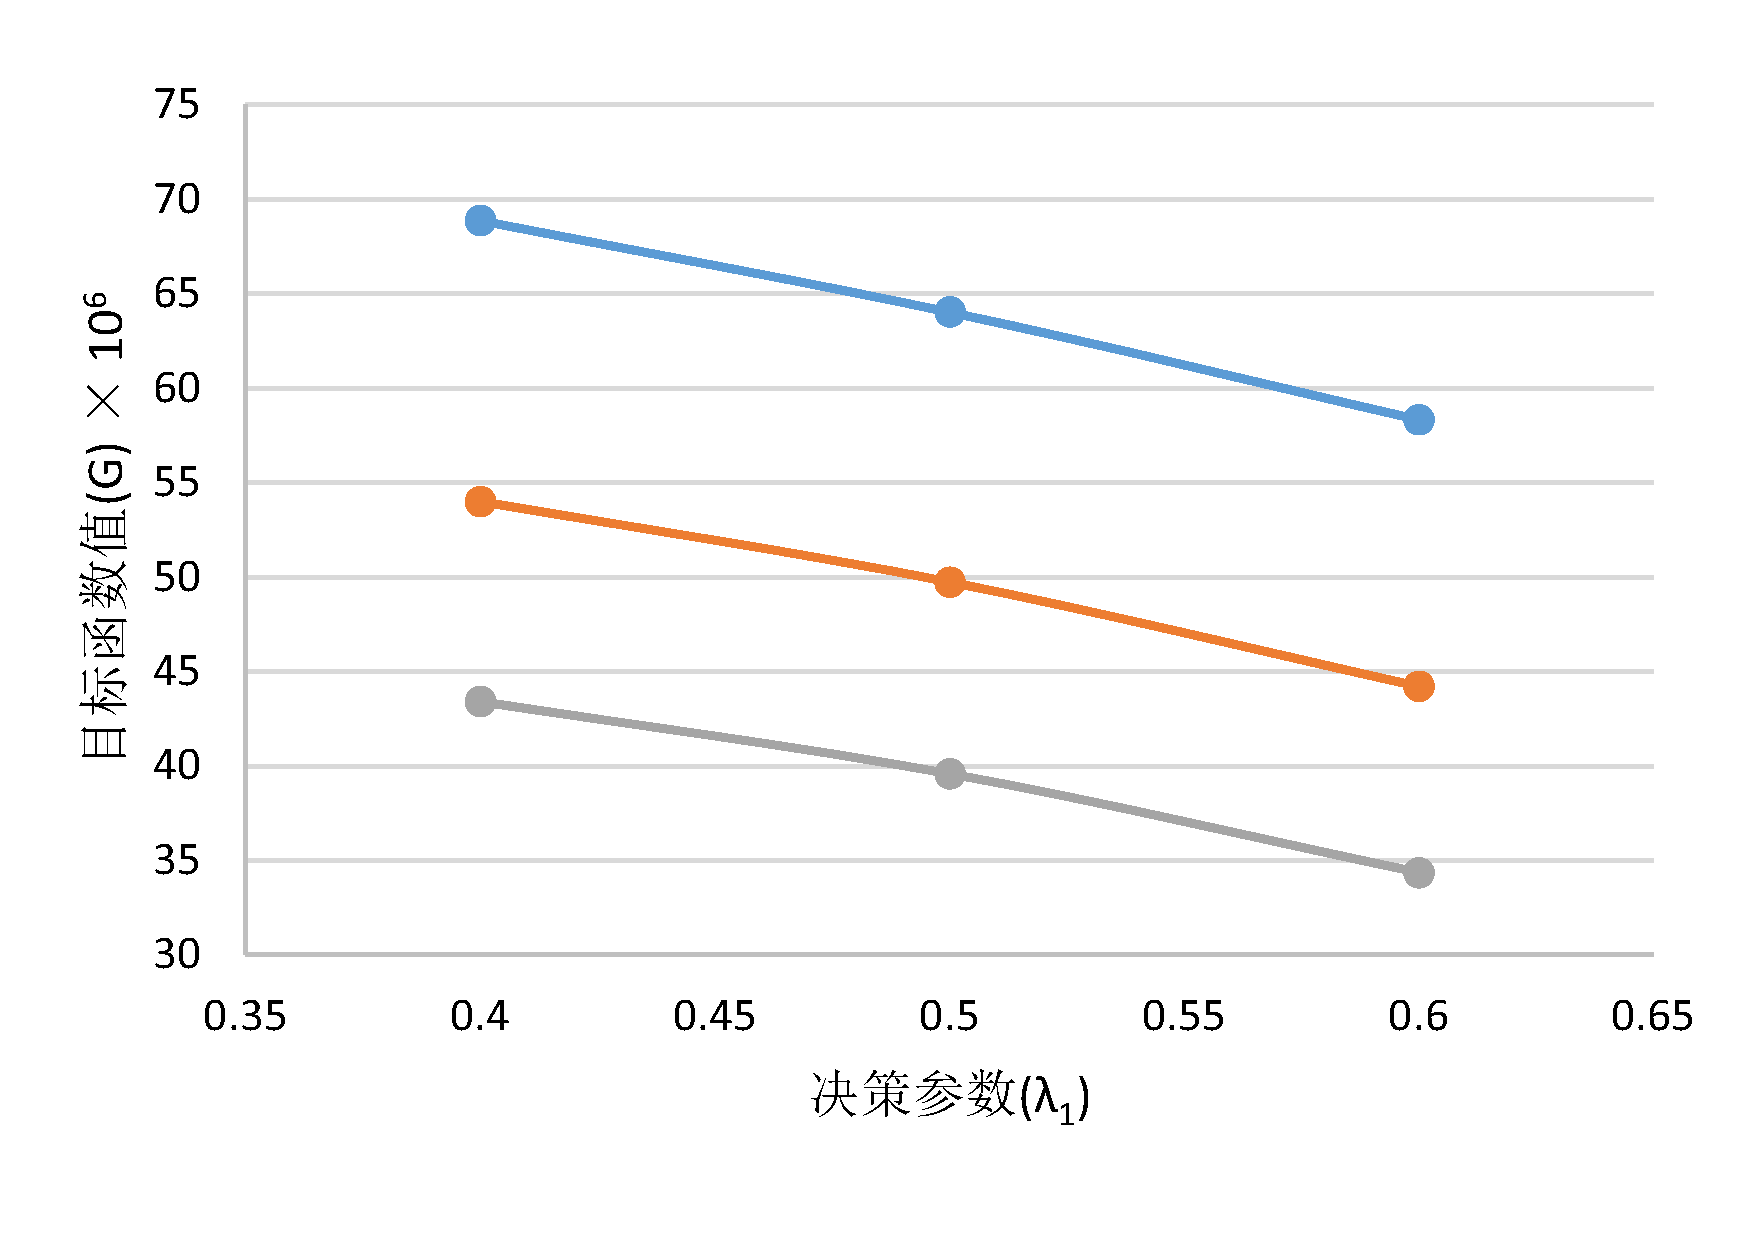
\includegraphics[height = 5.8cm, angle = -90,trim = 50 20 50 10]{alg_1_750}}
\subfloat[$n = 500$]{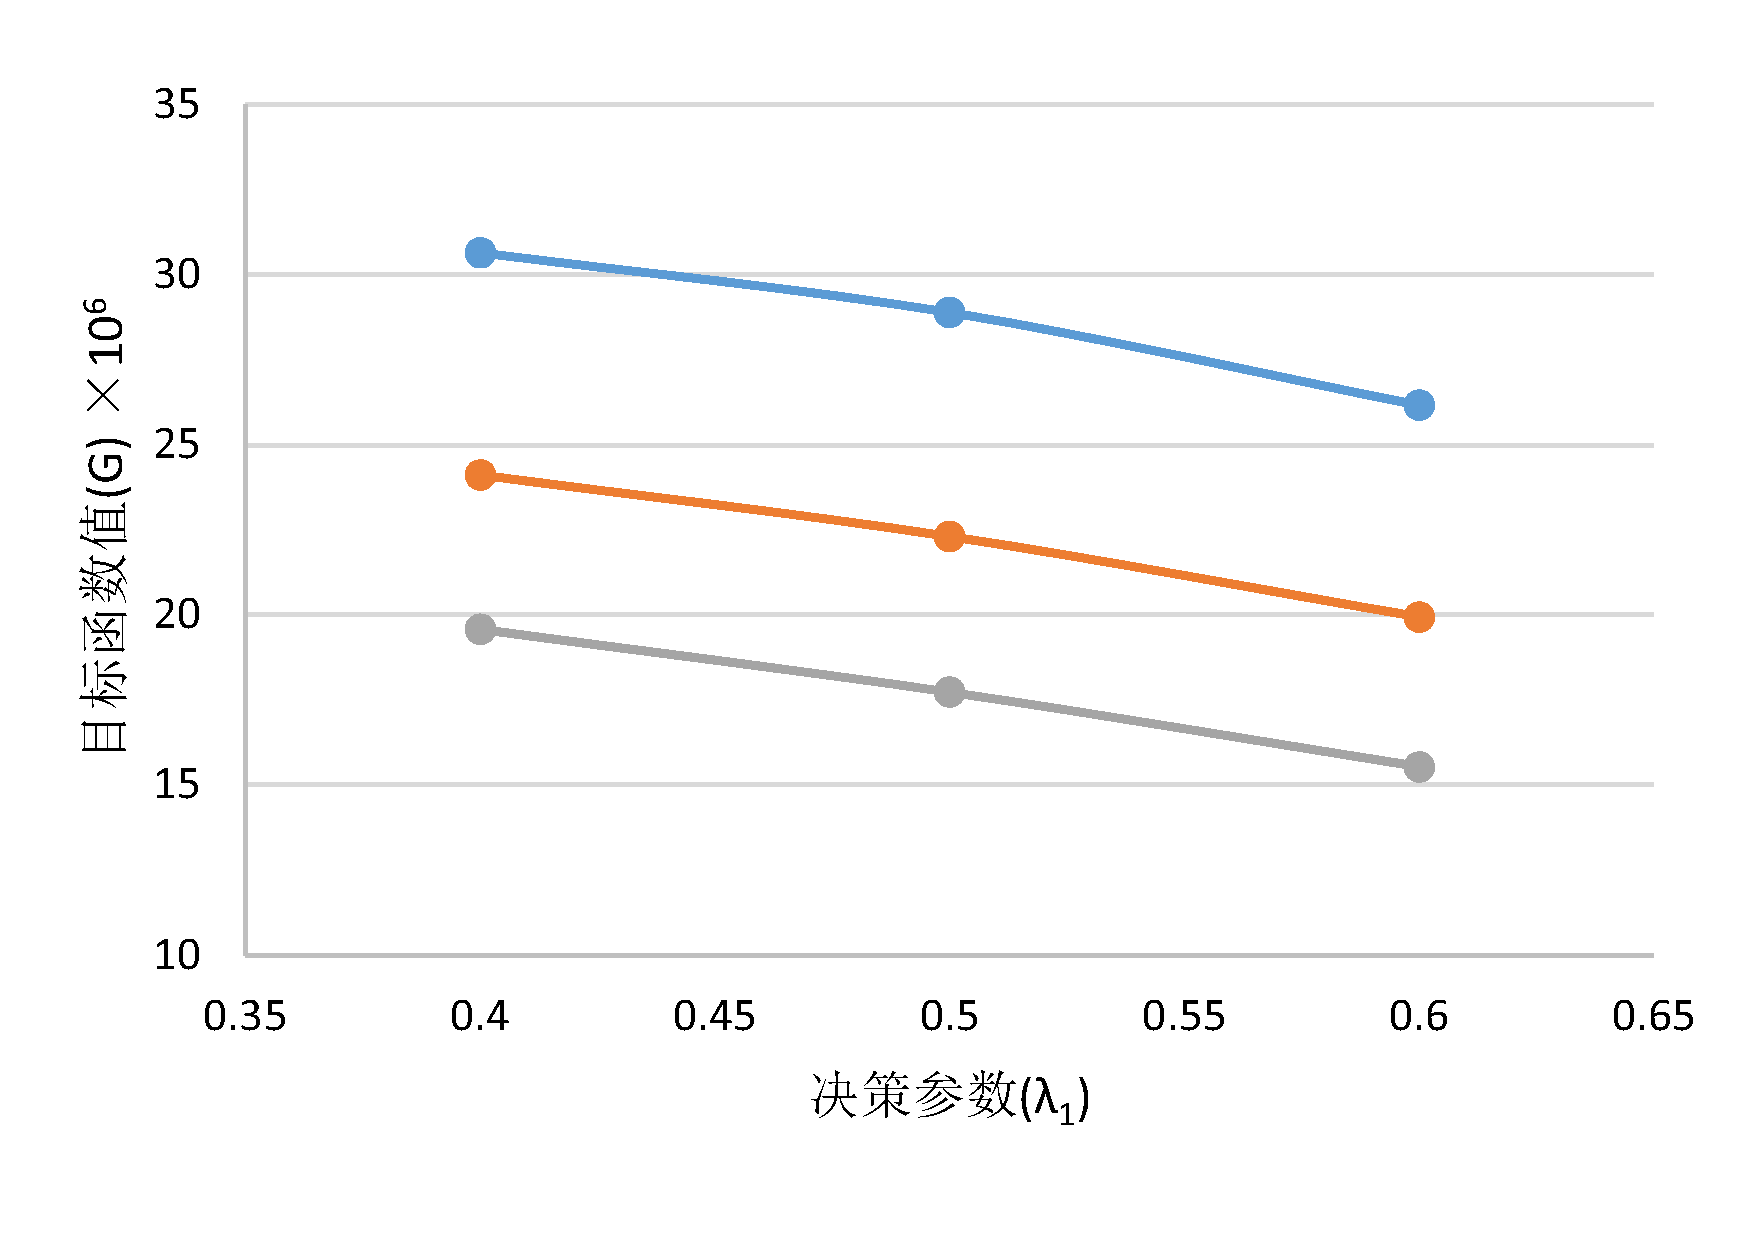
\includegraphics[height = 5.8cm, angle = -90,trim = 50 20 50 10]{alg_1_500}}\\
\end{figure}
\subsection{模型2}
\subsubsection{算法比较}
\subsubsection{权衡决策参数}
\subsubsection{流水线指标与评价}

\section{小结}